\documentclass[11pt,compress,t,notes=noshow, aspectratio=169, xcolor=table]{beamer}

\usepackage{../../style/lmu-lecture}
% Defines macros and environments
% This file is included in slides and exercises

% Rarely used fontstyle for R packages, used only in 
% - forests/slides-forests-benchmark.tex
% - exercises/single-exercises/methods_l_1.Rnw
% - slides/cart/attic/slides_extra_trees.Rnw
\newcommand{\pkg}[1]{{\fontseries{b}\selectfont #1}}

% Spacing helpers, used often (mostly in exercises for \dlz)
\newcommand{\lz}{\vspace{0.5cm}} % vertical space (used often in slides)
\newcommand{\dlz}{\vspace{1cm}}  % double vertical space (used often in exercises, never in slides)
\newcommand{\oneliner}[1] % Oneliner for important statements, used e.g. in iml, algods
{\begin{block}{}\begin{center}\begin{Large}#1\end{Large}\end{center}\end{block}}

% Don't know if this is used or needed, remove?
% textcolor that works in mathmode
% https://tex.stackexchange.com/a/261480
% Used e.g. in forests/slides-forests-bagging.tex
% [...] \textcolor{blue}{\tfrac{1}{M}\sum^M_{m} [...]
% \makeatletter
% \renewcommand*{\@textcolor}[3]{%
%   \protect\leavevmode
%   \begingroup
%     \color#1{#2}#3%
%   \endgroup
% }
% \makeatother


%\title{iML: Ante-hoc Methods for Neural Networks}
%\subtitle{Learning to explain}
\title{Interpretable Machine Learning}
\date{}

\begin{document}
%	\maketitle
	\graphicspath{ {./figure/} }

\newcommand{\titlefigure}{figure/bild16}
\newcommand{\learninggoals}{
\item Optimization problems in hard-masking
\item Generative masking
\item Sampling-based instance-wise feature selection}

\lecturechapter{Learning to Explain}
\lecture{Interpretable Machine Learning}

 
\begin{frame}[c]{Instance-wise Feature Selection}
    \begin{itemize}
        \item What happens when we do not have explanation data?
        \bigskip
        \item Need to use the task-specific supervision signal to create explanations
        \bigskip
        \item Key principle: Given an instance, automatically learn to select features during inference
from the task-specific supervised signal
    \end{itemize}
\end{frame}	
	
\begin{frame}{Instance-wise Feature Selection}
    \begin{itemize}
        \item Key principle: Given an instance, automatically learn to select features during inference
        \item The selected features can be implemented as a binary mask over the original feature
space
\item Selector network selects the mask, predictor network predicts using the masked input
    \end{itemize}
    \begin{figure}
        \centering
        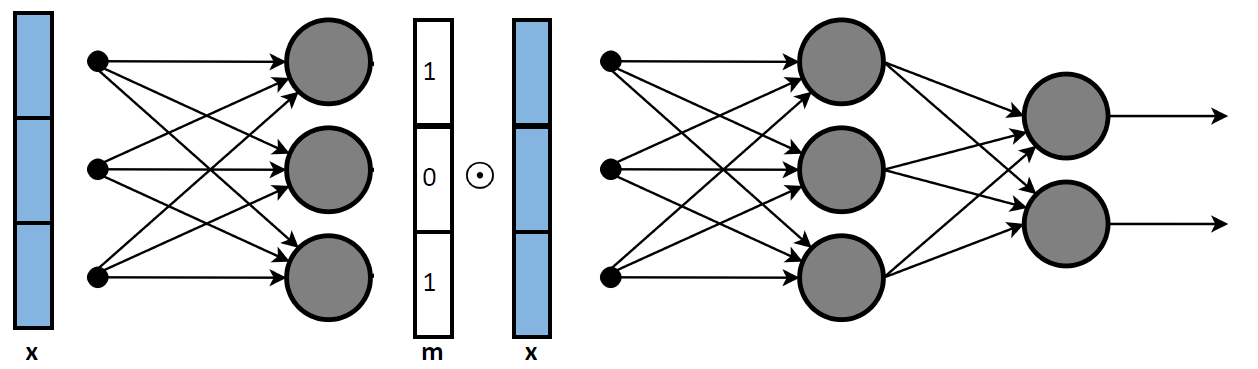
\includegraphics[scale=.45]{bild16}
    \end{figure}
\end{frame}
	
	
\begin{frame}{Problems in optimisation}
    \begin{itemize}
        \item Selector network selects the mask, predictor network predicts using the masked input
        \item Binary masking introduces discontinuity in the neural network
\item Discontinuity $\rightarrow$ gradient-based optimisation is not possible
\bigskip
\item How can we learn the parameters of such a network using gradient-based optimization?
    \end{itemize}
    \begin{figure}
        \centering
        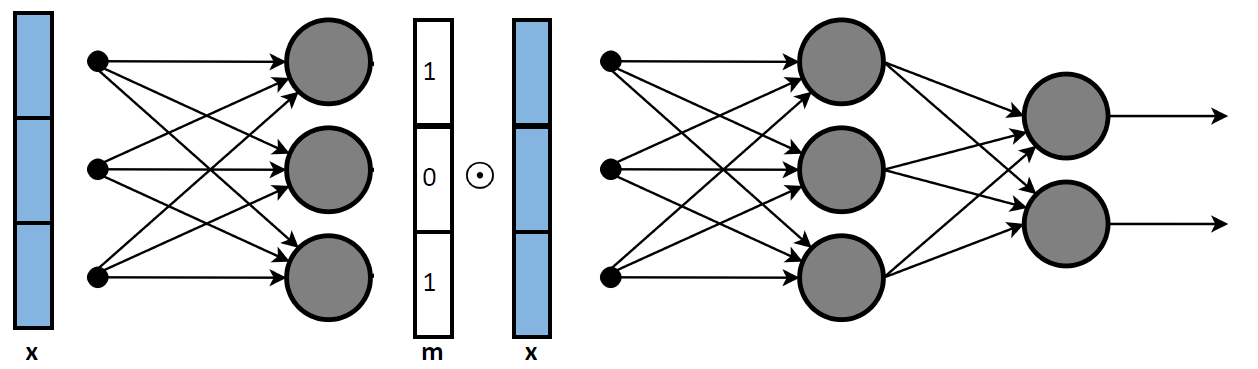
\includegraphics[scale=.43]{bild16}
    \end{figure}
\end{frame}	

\begin{frame}{Generative masks}
    \begin{itemize}
        \item Masks are generated from a probability distribution
        \item Instance-wise feature selection as finding the expectation of the predictor function
distributed according to human interpretability
    \end{itemize}
    \bigskip
   \begin{equation*}
             \centering
    \mathcal{F}(\boldsymbol{\theta}):=\int p(\mathbf{m} ; \mathbf{x}, \boldsymbol{\theta}) f(\mathbf{m} \odot \mathbf{x} ; \boldsymbol{\phi}) \mathrm{d} \mathbf{x}=\mathbb{E}_{p(\mathbf{m} ; \mathbf{x}, \boldsymbol{\theta})}[f(\mathbf{m} \odot \mathbf{x} ; \boldsymbol{\phi})]
\end{equation*}
    
    
    
    %\begin{figure}
     %   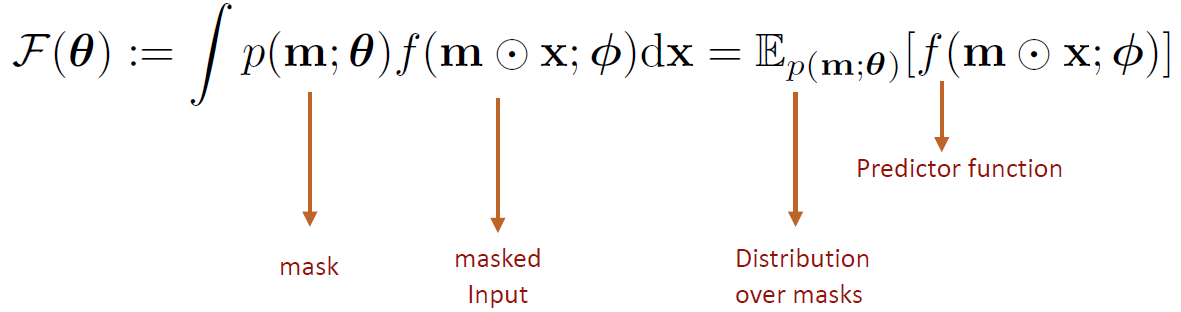
\includegraphics[scale=.4]{bild17}
    %\end{figure}
\end{frame}
	
	
\begin{frame}{Instance-wise Feature Selection}
\begin{itemize}
    \item The distribution over explanations is parameterized by a neural network
    \item The predictor network is also parameterized by a neural network
\end{itemize}
\bigskip
\begin{equation*}
             \centering
    \mathcal{F}(\boldsymbol{\theta}):=\int p(\mathbf{m} ; \boldsymbol{\theta}) f(\mathbf{m} \odot \mathbf{x} ; \boldsymbol{\phi}) \mathrm{d} \mathbf{x}=\mathbb{E}_{p(\mathbf{m} ; \boldsymbol{\theta})}[f(\mathbf{m} \odot \mathbf{x} ; \boldsymbol{\phi})]
\end{equation*}

\bigskip

%\begin{figure}
%    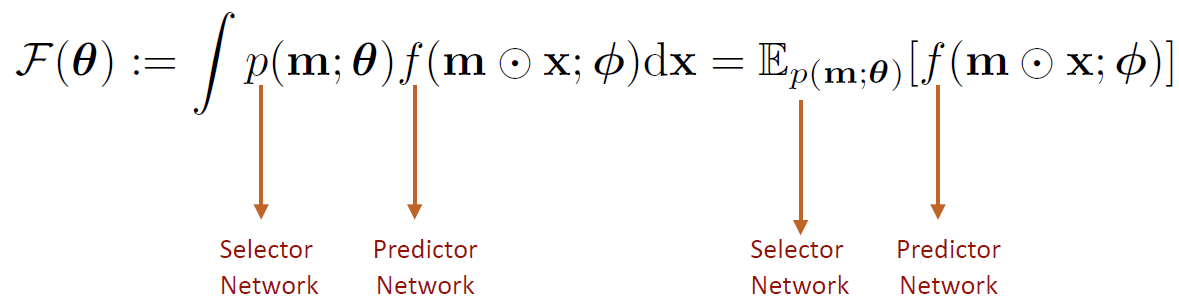
\includegraphics[scale=.4]{bild18}
%\end{figure}
\begin{itemize}
    \item Predictor network accepts a masked input
\end{itemize}
\end{frame}

\begin{frame}{Monte Carlo Sampling}
 
$$
\mathcal{F}(\boldsymbol{\theta}):=\int p(\mathbf{m} ; \mathbf{x}, \boldsymbol{\theta}) f(\mathbf{m} \odot \mathbf{x} ; \boldsymbol{\phi}) \mathrm{d} \mathbf{x}=\mathbb{E}_{p(\mathbf{m} ; \mathbf{x}, \boldsymbol{\theta})}[f(\mathbf{m} \odot \mathbf{x} ; \boldsymbol{\phi})] 
$$


    \begin{itemize}
        \item \textbf{Trick:} $\nabla_{\boldsymbol{\theta}} \log p(\mathbf{x} ; \boldsymbol{\theta})=\frac{\nabla_{\boldsymbol{\theta}} p(\mathbf{x} ; \boldsymbol{\theta})}{p(\mathbf{x} ; \boldsymbol{\theta})}$
    \end{itemize}
\medskip

$\leadsto$ In a simplified notation (ignoring $\mathbf{m}$), we get the following:
$$
\smallskip
    \begin{aligned}
        \,\,\,\,\,\,\,\,\,\,\,\,\,\,\,\,
        \boldsymbol{\eta}:=\nabla_{\boldsymbol{\theta}} \mathcal{F}(\boldsymbol{\theta}) &=\nabla_{\boldsymbol{\theta}} \mathbb{E}_{p(\mathbf{x} ; \boldsymbol{\theta})}[f(\mathbf{x} ; \boldsymbol{\phi})] \\
        &=\nabla_{\boldsymbol{\theta}} \int p(\mathbf{x} ; \boldsymbol{\theta}) f(\mathbf{x}) d \mathbf{x}=\int f(\mathbf{x}) \nabla_{\boldsymbol{\theta}} p(\mathbf{x} ; \boldsymbol{\theta}) d \mathbf{x} \\
        &=\int p(\mathbf{x} ; \boldsymbol{\theta}) f(\mathbf{x}) \nabla_{\boldsymbol{\theta}} \log p(\mathbf{x} ; \boldsymbol{\theta}) d \mathbf{x} \\
        &=\mathbb{E}_{p(\mathbf{x} ; \boldsymbol{\theta})}\left[f(\mathbf{x}) \nabla_{\boldsymbol{\theta}} \log p(\mathbf{x} ; \boldsymbol{\theta})\right]
    \end{aligned}
$$
\end{frame}

\begin{frame}{Monte Carlo Estimator}
   
\begin{equation*}
     \mathcal{F}(\boldsymbol{\theta}):=\int p(\mathbf{m} ; \mathbf{x}, \boldsymbol{\theta}) f(\mathbf{m} \odot \mathbf{x} ; \boldsymbol{\phi}) \mathrm{d} \mathbf{x}=\mathbb{E}_{p(\mathbf{m} ; \mathbf{x}, \boldsymbol{\theta})}[f(\mathbf{m} \odot \mathbf{x} ; \boldsymbol{\phi})]
\end{equation*}

$$
\begin{aligned}
\boldsymbol{\eta}:=\nabla_{\boldsymbol{\theta}} \mathcal{F}(\boldsymbol{\theta})=\nabla_{\boldsymbol{\theta}} \mathbb{E}_{p(\mathbf{x} ; \boldsymbol{\theta})}[f(\mathbf{x} ; \boldsymbol{\phi})] &=\mathbb{E}_{p(\mathbf{x} ; \boldsymbol{\theta})}\left[f(\mathbf{x}) \nabla_{\boldsymbol{\theta}} \log p(\mathbf{x} ; \boldsymbol{\theta})\right] \\
&=\frac{1}{N} \sum_{n=1}^N f\left(\hat{\mathbf{x}}^{(n)}\right) \nabla_{\boldsymbol{\theta}} \log p\left(\hat{\mathbf{x}}^{(n)} ; \boldsymbol{\theta}\right) ; \quad \hat{\mathbf{x}}^{(n)} \sim p(\mathbf{x} ; \boldsymbol{\theta})
\end{aligned}
$$

%\begin{figure}
%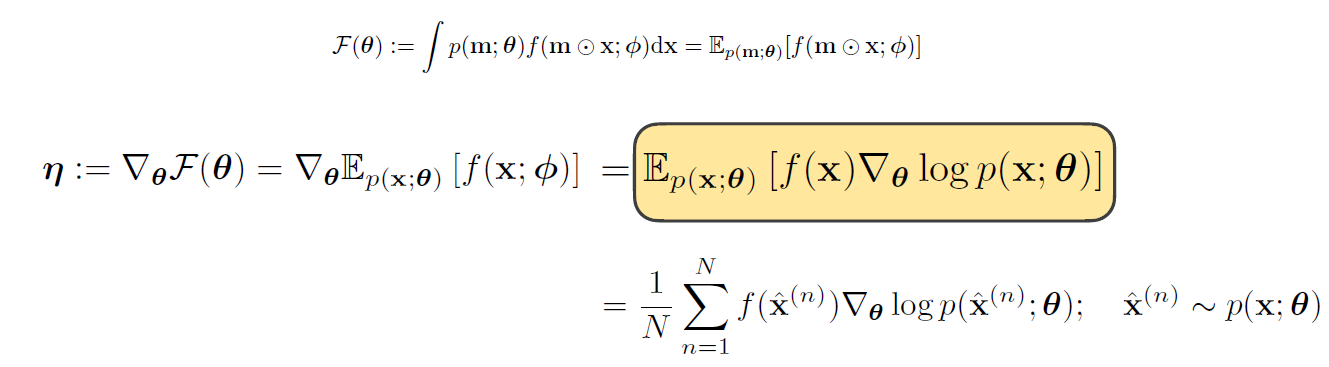
\includegraphics[scale=.35]{bild20}
%\end{figure}


    \begin{itemize}
        \item Sample N masks from the probability distribution p
        \item Compute the weighted avg. of the samples where:
        \begin{itemize}
            \item weight = derivative of the log prob. of the sample mask
        \end{itemize}
        \item update the parameters of the selector network using this weighted average
    \end{itemize}
\end{frame}

\begin{frame}{Reducing variance}
  
  \begin{equation*}
     \mathcal{F}(\boldsymbol{\theta}):=\int p(\mathbf{m} ; \mathbf{x}, \boldsymbol{\theta}) f(\mathbf{m} \odot \mathbf{x} ; \boldsymbol{\phi}) \mathrm{d} \mathbf{x}=\mathbb{E}_{p(\mathbf{m} ; \mathbf{x}, \boldsymbol{\theta})}[f(\mathbf{m} \odot \mathbf{x} ; \boldsymbol{\phi})]
\end{equation*}

  \bigskip
  \begin{itemize}
      \item Monte Carlo estimators suffer from the problem of high variance
      \item Solution: introduce a constant baseline value $\beta$
  \end{itemize}
  \bigskip
 
 
 \begin{equation*}
     \eta = \mathbb{E}_{p(x;\theta)}[(f(x) - \beta)\nabla_\theta \log p(x;\theta)]
 \end{equation*} 
  
 % \begin{figure}
%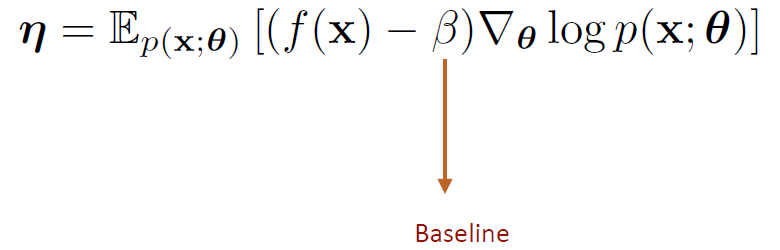
\includegraphics[scale=.5]{bild21}
%  \end{figure}
  
  
\end{frame}

\begin{frame}[c]{Conclusion}
    \begin{itemize}
        \item Prefer simple models for better interpretability
        \item Regularisation for enforcing sparsity in the parameter space
        \item Feature selection for enforcing sparsity in the feature space
        \item Instance-wise feature selection selects different features based on different instances
        \item Selector and predictor architecture for instance-wise feature selection
        \item Optimisation using without explanation data requires tricks like Monte-Carlo sampling
with gradients
    \end{itemize}
\end{frame}

\begin{frame}[c]{References}
    \begin{itemize}
        \item “Learning to Explain: An Information-Theoretic Perspective on Model Interpretation” — J.
Chen, Song, M.J. Wainwright, M. I. Jordan. ICML 2018.
\begin{itemize}
    \item \url{http://proceedings.mlr.press/v80/chen18j/chen18j.pdf}
\end{itemize}
\bigskip
\item “Explain and Predict, and then Predict again" — Z Zhang, K Rudra, A Anand. WSDM 2020.
\begin{itemize}
    \item \url{https://arxiv.org/pdf/2101.04109.pdf}
\end{itemize}
\bigskip
\item “INVASE: Instance-wise Variable Selection using Neural Networks” J. Yoon, J. Jordon, M.
Schaar. ICLR 2019.
\begin{itemize}
    \item \url{https://openreview.net/pdf?id=BJg_roAcK7}
\end{itemize}
    \end{itemize}
\end{frame}
\endlecture
\end{document}	